\chapter{Preventivo}

\section{Verso la RTB}

\subsection{Primo periodo}

In questa fase i ruoli da ricoprire per portare a termine gli obiettivi
pianificati sono:
\begin{itemize}
    \item \textit{Responsabile};
    \item \textit{Amministratore};
    \item \textit{Verificatore}.
\end{itemize}

\subsubsection{Preventivo orario}

\begin{table}[!ht]
    \centering
    \begin{tabular}{|l|c|c|c|c|c|c|c|}
    \hline
    \textbf{Membro} & \multicolumn{1}{l|}{\textbf{RE}} & \multicolumn{1}{l|}{\textbf{AM}} & \multicolumn{1}{l|}{\textbf{AN}} & \multicolumn{1}{l|}{\textbf{PT}} & \multicolumn{1}{l|}{\textbf{PR}} & \multicolumn{1}{l|}{\textbf{VE}} & \multicolumn{1}{l|}{\textbf{Totale ore persona}} \\ \hline
    \textit{Marco Mazzucato}  & 2 & 3  & - & - & - & 1 & 6  \\ \hline
    \textit{Marco Mamprin}    & - & 3  & - & - & - & 1 & 4  \\ \hline
    \textit{Marko Vukovic}    & 2 & 3  & - & - & - & 1 & 6  \\ \hline
    \textit{Mattia Zanellato} & - & 3  & - & - & - & 1 & 4  \\ \hline
    \textit{Emanuele Pase}    & - & 3  & - & - & - & 1 & 4  \\ \hline
    \textit{Riccardo Contin}  & - & 3  & - & - & - & 1 & 4  \\ \hline
    \textit{Lorenzo Onelia}   & - & 3  & - & - & - & 1 & 4  \\ \hline
    \textbf{Totale ore ruolo} & 4 & 21 & - & - & - & 7 & 32 \\ \hline
    \end{tabular}
    \caption{Distribuzione delle ore per la prima milestone}
\end{table}

\begin{figure}[!ht]
    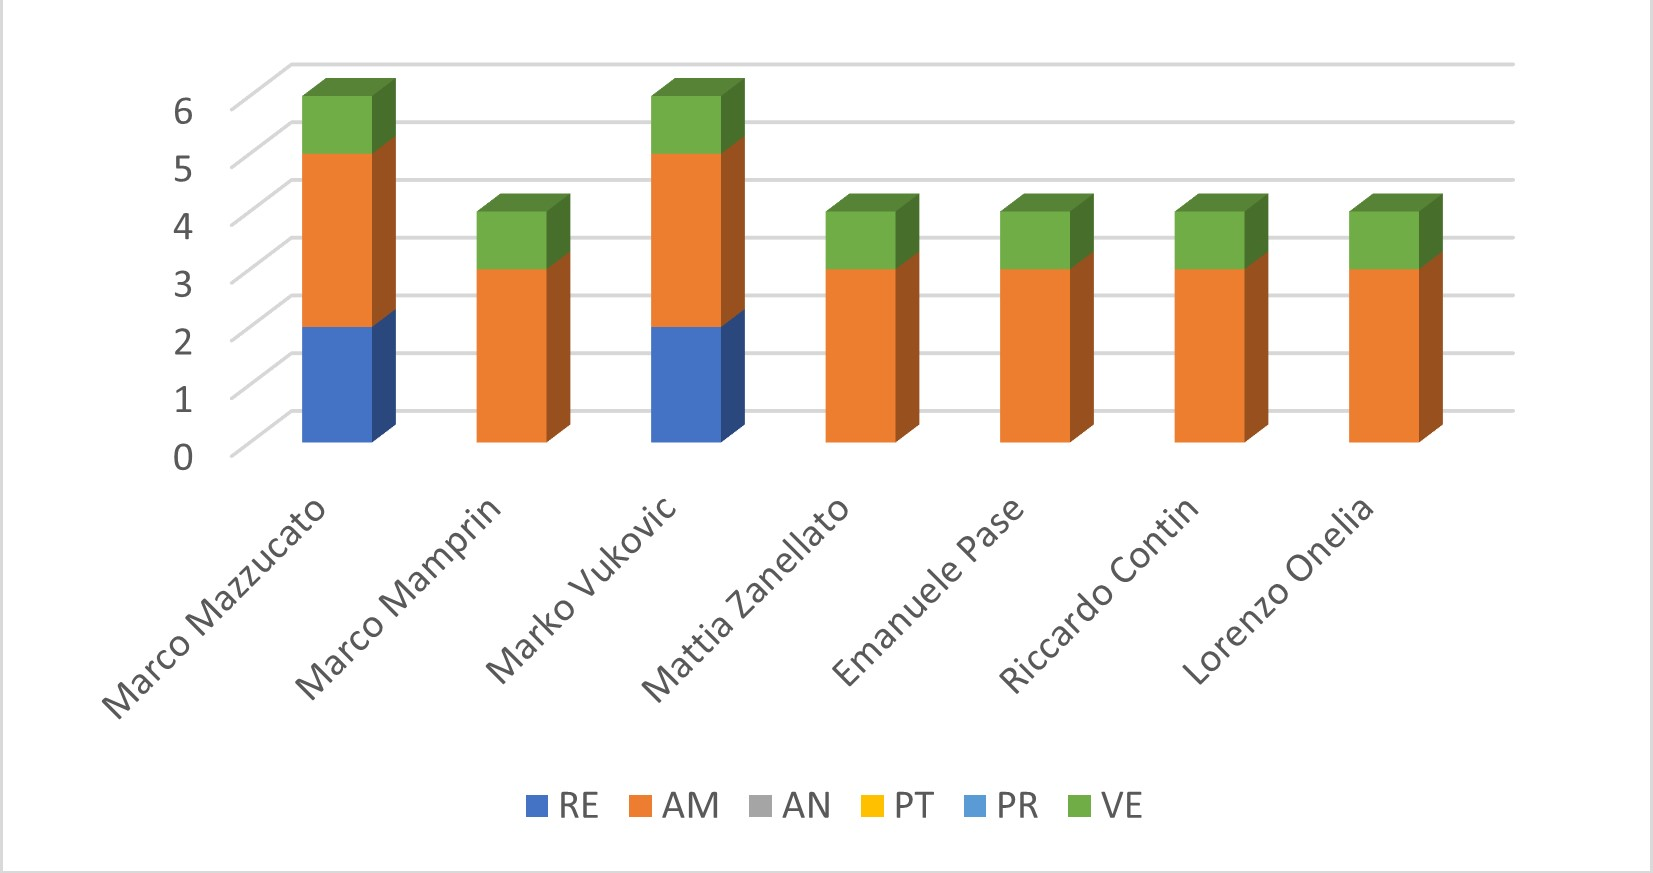
\includegraphics[width=1.0\textwidth]{Istogramma1.jpg}
    \caption{Istogramma della distribuzione delle ore} 
\end{figure}

\begin{figure}[!ht]
    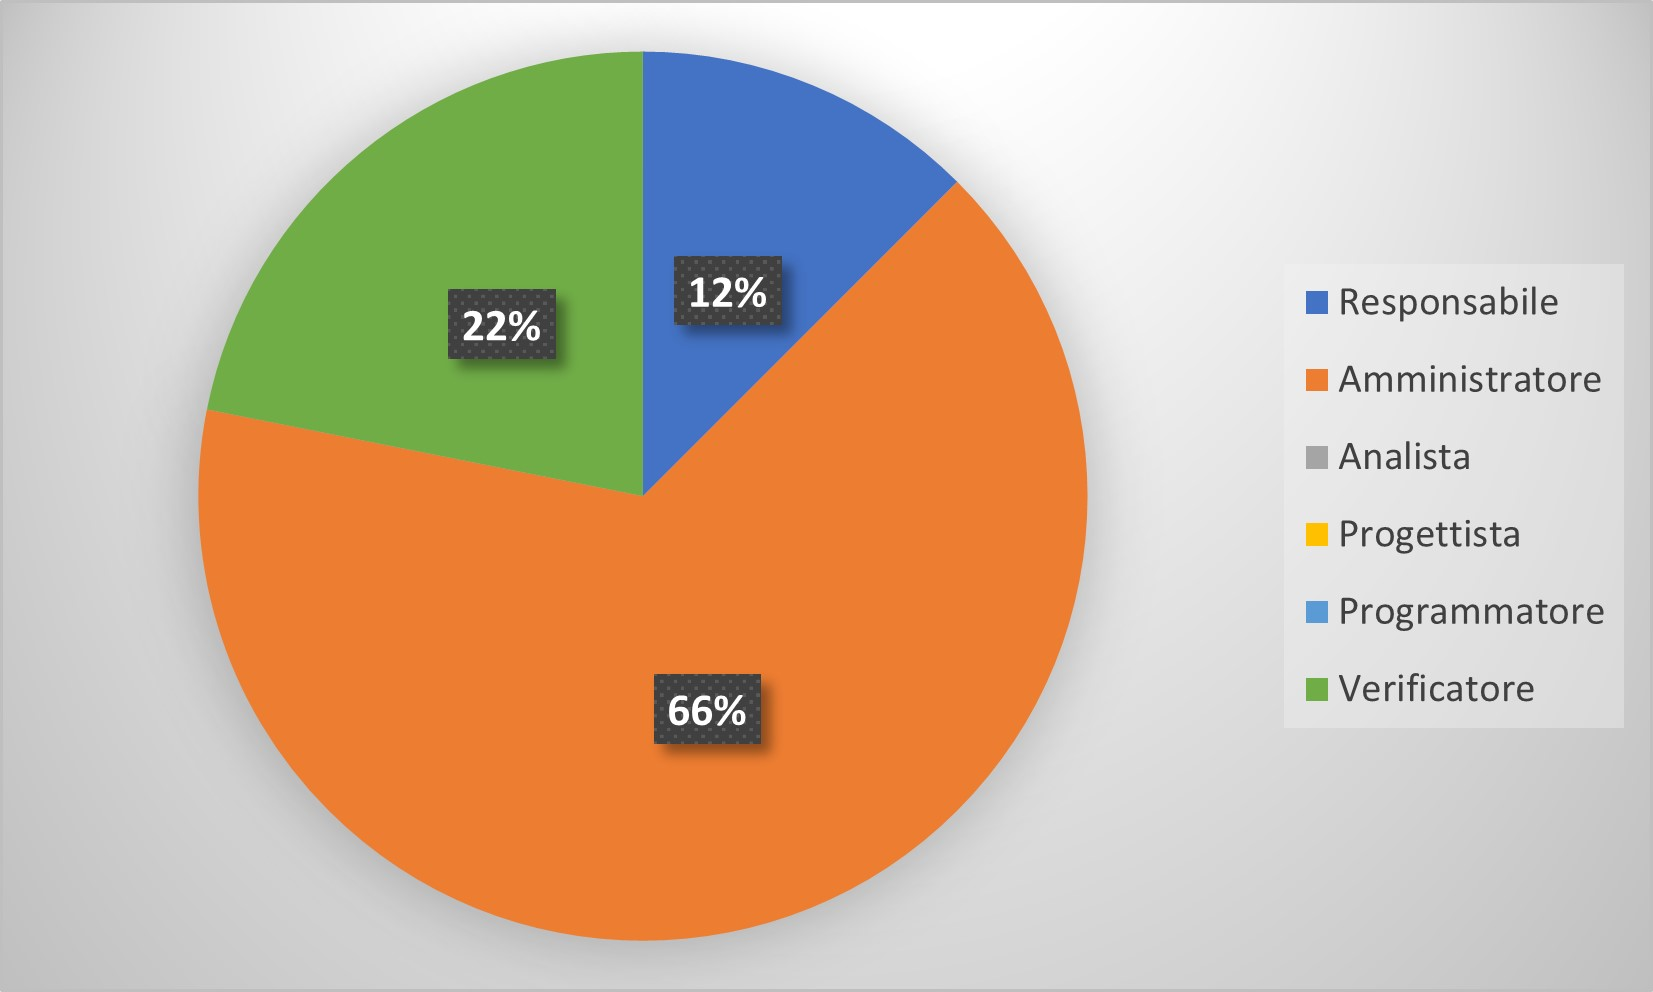
\includegraphics[width=1.0\textwidth]{Torta1.1.jpg}
    \caption{Grafico a torta della distribuzione delle ore} 
\end{figure}

\newpage
\subsubsection{Preventivo economico}

\begin{table}[!ht]
    \centering
    \begin{tabular}{|l|c|c|}
    \hline
    \textbf{Ruolo} & \multicolumn{1}{l|}{\textbf{Ore}} & \multicolumn{1}{l|}{\textbf{Costo (€)}} \\ \hline
    \textit{Responsabile} & 4 & 120 \\ \hline
    \textit{Amministratore} & 21 & 420 \\ \hline
    \textit{Analista} & - & - \\ \hline
    \textit{Progettista} & - & - \\ \hline
    \textit{Programmatore} & - & - \\ \hline
    \textit{Verificatore} & 7 & 105 \\ \hline
    \textbf{Totale} & 32 & 645 \\ \hline
    \end{tabular}
    \caption{Prospetto dei costi per la prima milestone}
\end{table}

\begin{figure}[!ht]
    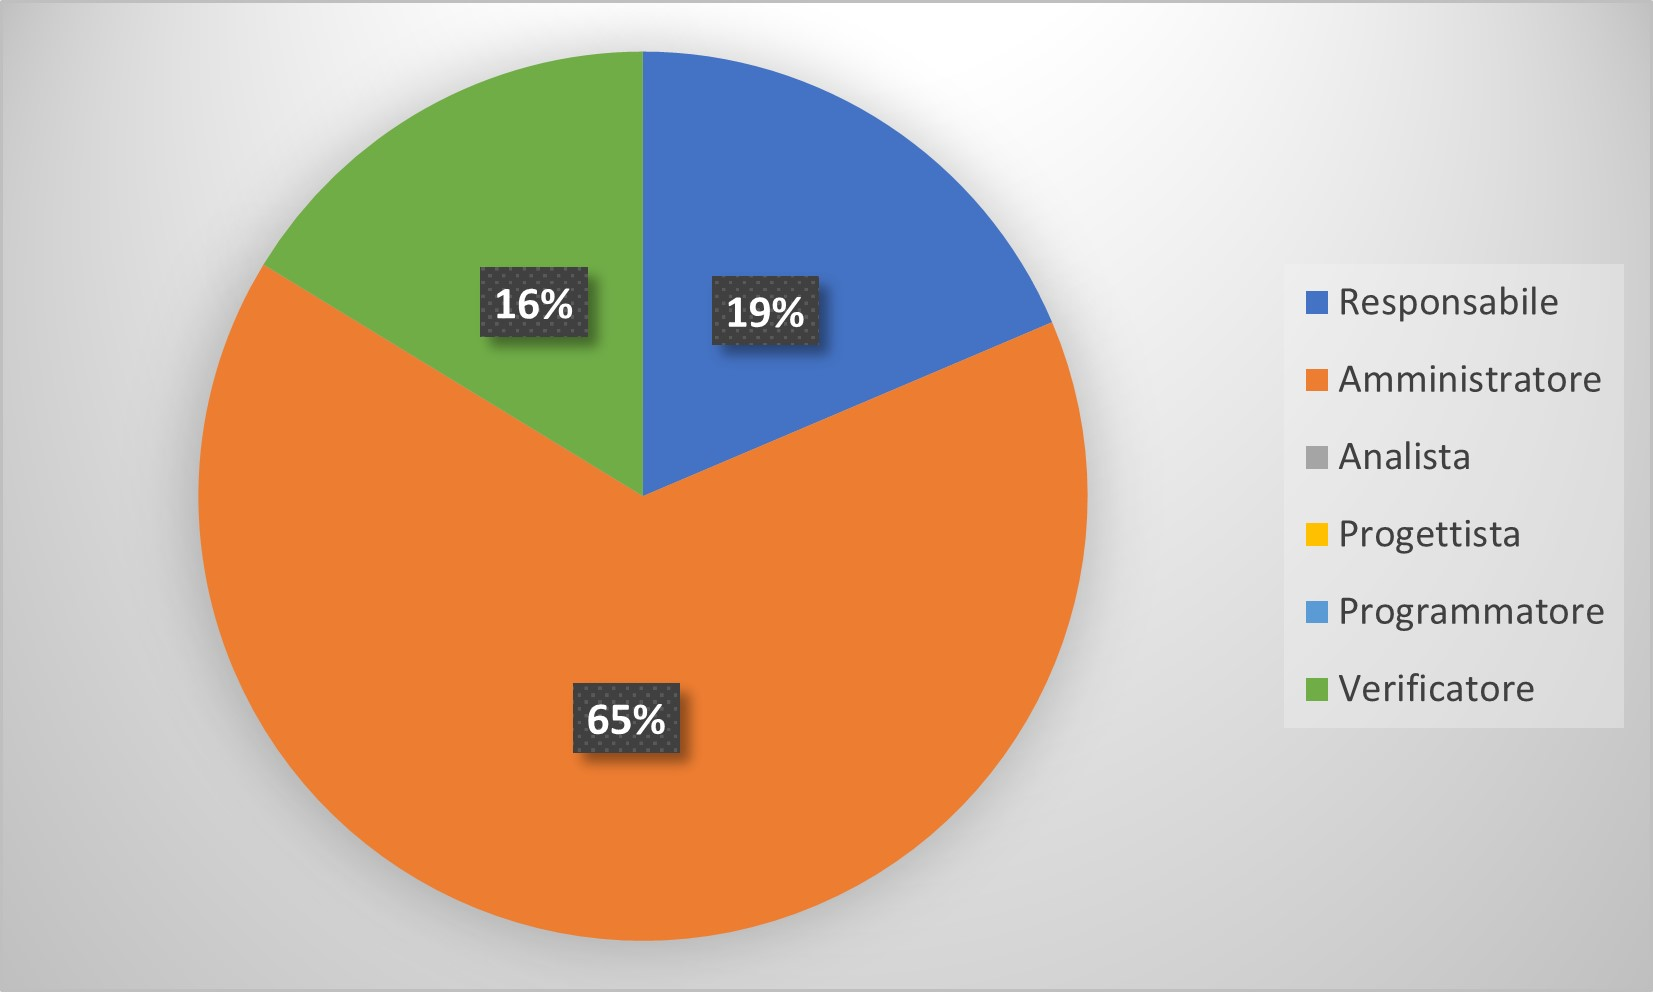
\includegraphics[width=1.0\textwidth]{Torta1.2.jpg}
    \caption{Grafico a torta della distribuzione dei costi} 
\end{figure}

\newpage
\subsection{Secondo periodo}

In questa fase i ruoli da ricoprire per portare a termine gli obiettivi
pianificati sono:
\begin{itemize}
    \item \textit{Responsabile};
    \item \textit{Amministratore};
    \item \textit{Analista};
    \item \textit{Verificatore}.
\end{itemize}

\subsubsection{Preventivo orario}

\begin{table}[!ht]
    \centering
    \begin{tabular}{|l|c|c|c|c|c|c|c|}
    \hline
    \textbf{Membro} & \multicolumn{1}{l|}{\textbf{RE}} & \multicolumn{1}{l|}{\textbf{AM}} & \multicolumn{1}{l|}{\textbf{AN}} & \multicolumn{1}{l|}{\textbf{PT}} & \multicolumn{1}{l|}{\textbf{PR}} & \multicolumn{1}{l|}{\textbf{VE}} & \multicolumn{1}{l|}{\textbf{Totale ore persona}} \\ \hline
    \textit{Marco Mazzucato}  & - & 2  & 2  & - & - & 3  & 7  \\ \hline
    \textit{Marco Mamprin}    & - & 2  & 1  & - & - & 2  & 5  \\ \hline
    \textit{Marko Vukovic}    & - & -  & 4  & - & - & 3  & 7  \\ \hline
    \textit{Mattia Zanellato} & - & -  & 4  & - & - & 3  & 7  \\ \hline
    \textit{Emanuele Pase}    & - & -  & 4  & - & - & 3  & 7  \\ \hline
    \textit{Riccardo Contin}  & 4 & -  & 3  & - & - & 1  & 8  \\ \hline
    \textit{Lorenzo Onelia}   & - & 2  & 2  & - & - & 3  & 7  \\ \hline
    \textbf{Totale ore ruolo} & 4 & 6  & 20 & - & - & 18 & 48 \\ \hline
    \end{tabular}
    \caption{Distribuzione delle ore per la seconda milestone}
\end{table}

\begin{figure}[!ht]
    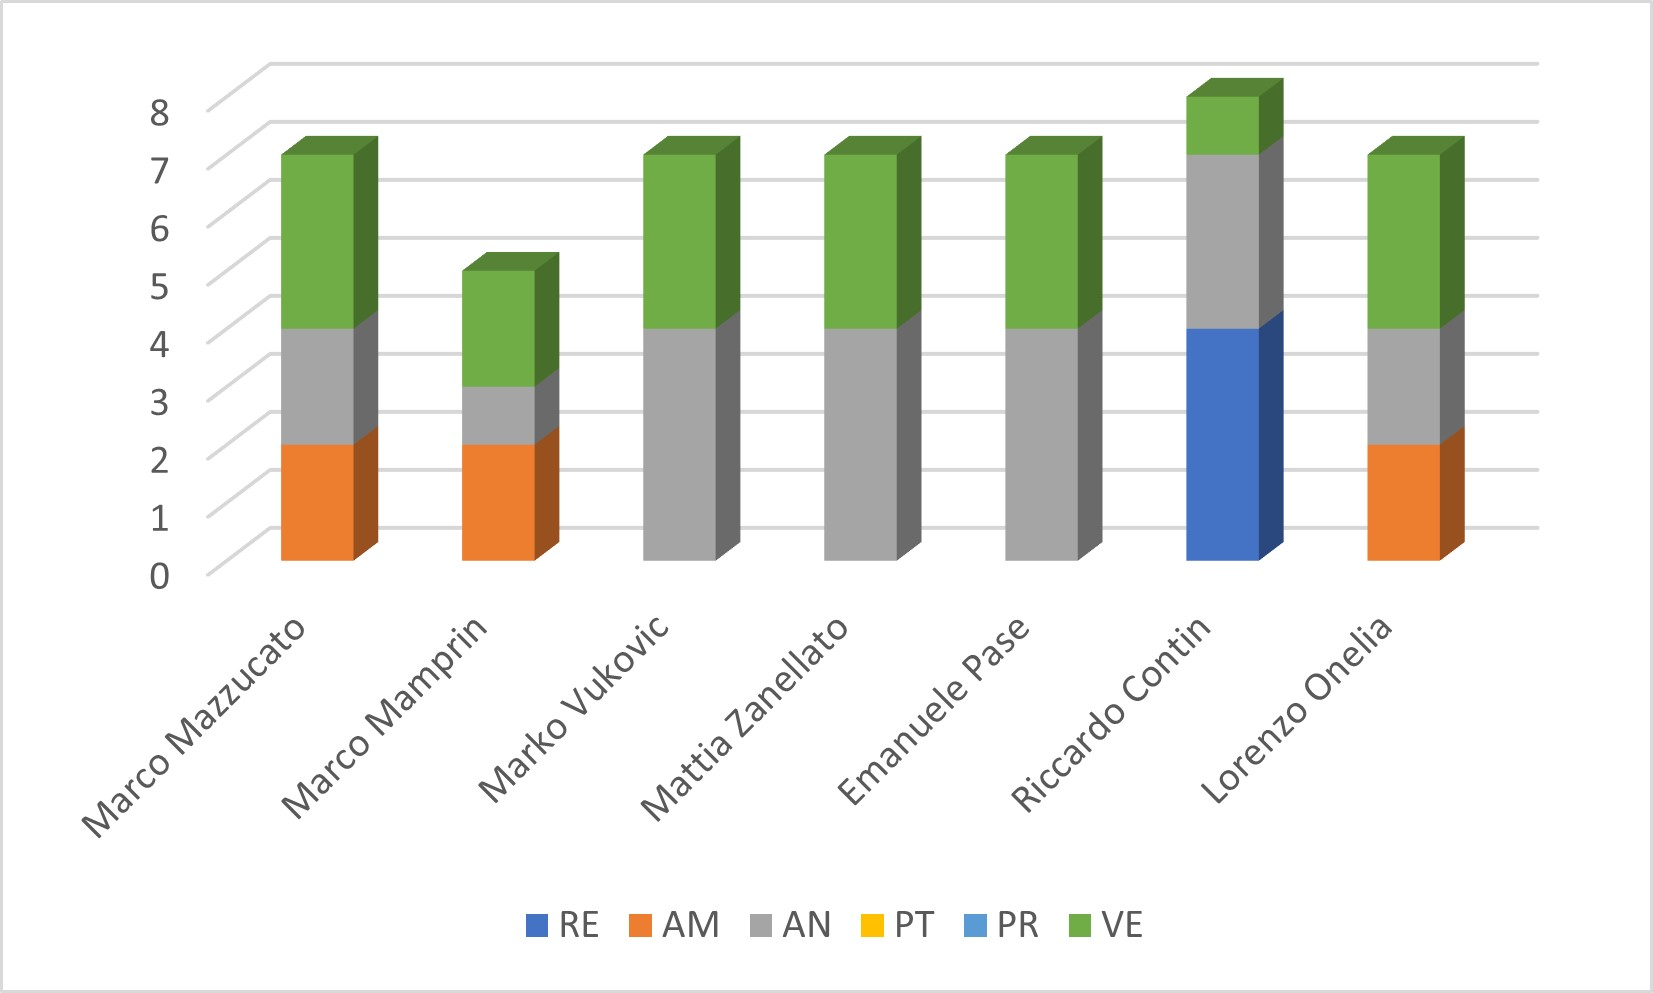
\includegraphics[width=1.0\textwidth]{Istogramma2.jpg}
    \caption{Istogramma della distribuzione delle ore} 
\end{figure}

\begin{figure}[!ht]
    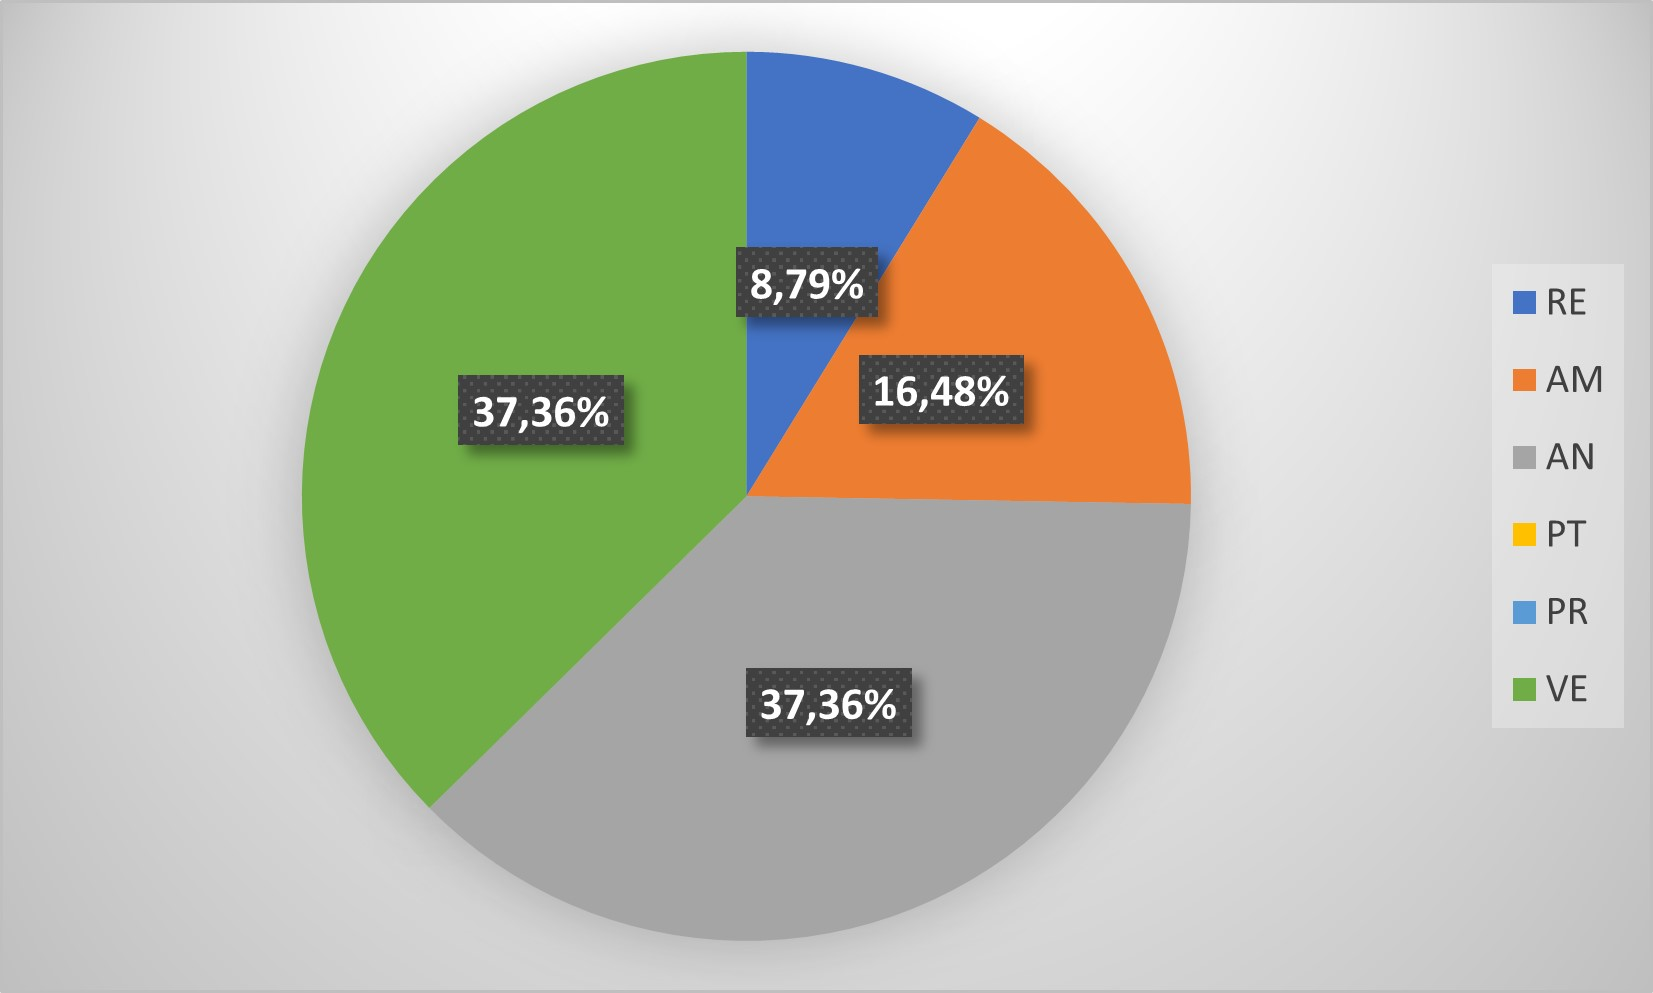
\includegraphics[width=1.0\textwidth]{Torta2.1.jpg}
    \caption{Grafico a torta della distribuzione delle ore} 
\end{figure}

\newpage
\subsubsection{Preventivo economico}

\begin{table}[!ht]
    \centering
    \begin{tabular}{|l|c|c|}
    \hline
    \textbf{Ruolo} & \multicolumn{1}{l|}{\textbf{Ore}} & \multicolumn{1}{l|}{\textbf{Costo (€)}} \\ \hline
    \textit{Responsabile} & 4 & 120 \\ \hline
    \textit{Amministratore} & 6 & 120 \\ \hline
    \textit{Analista} & 20 & 500 \\ \hline
    \textit{Progettista} & - & - \\ \hline
    \textit{Programmatore} & - & - \\ \hline
    \textit{Verificatore} & 18 & 270 \\ \hline
    \textbf{Totale} & 48 & 1010 \\ \hline
    \end{tabular}
    \caption{Prospetto dei costi per la seconda milestone}
\end{table}

\begin{figure}[!ht]
    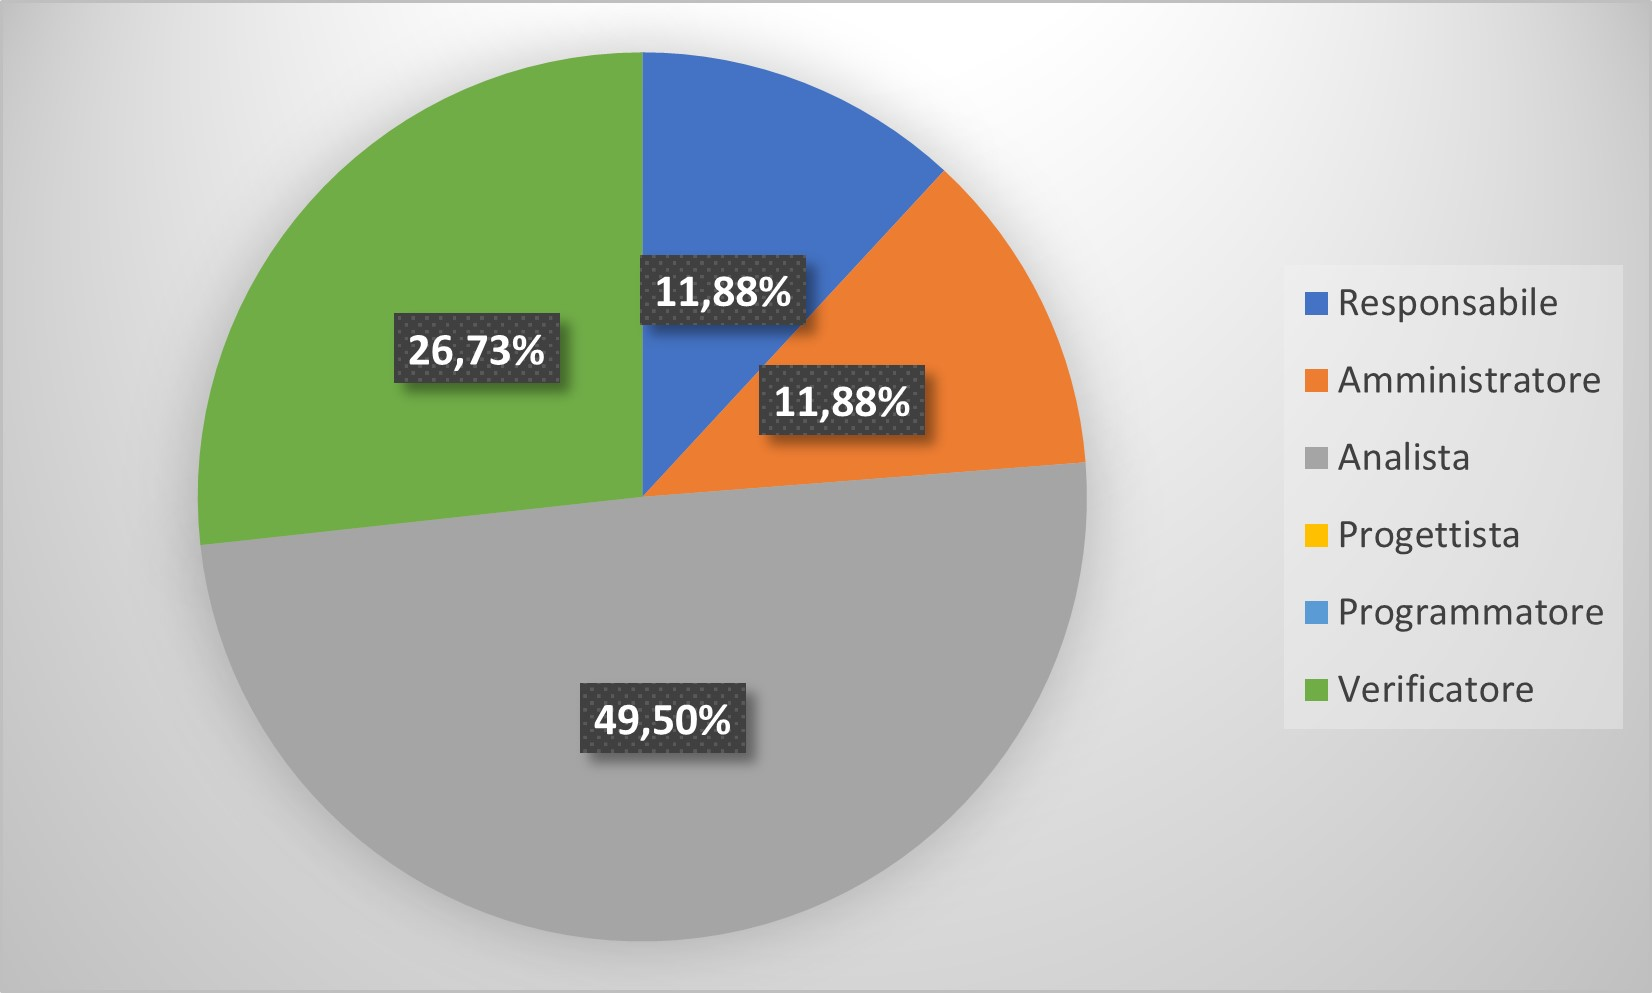
\includegraphics[width=1.0\textwidth]{Torta2.2.jpg}
    \caption{Grafico a torta della distribuzione dei costi} 
\end{figure}

\newpage
\subsection{Terzo periodo}

\section{Verso la PB}

\section{Verso la CA}